\documentclass[aspectratio=169]{beamer}

% ---------------------------------------------------------------------------
% Fonts (XeLaTeX) — Segoe UI, matching the web app's font stack
%   (body { font-family: Inter, system-ui, ..., "Segoe UI", sans-serif; })
% ---------------------------------------------------------------------------
\usepackage{fontspec}
\setmainfont{Segoe UI}
\setsansfont{Segoe UI}

\usepackage{amsmath}
\usepackage{tikz}
\usetikzlibrary{arrows.meta, positioning, shapes.misc}
\usepackage{graphicx}
\usepackage{booktabs}
\usepackage{enumitem}

% ---------------------------------------------------------------------------
% Palette — lifted directly from frontend/src/styles/variables.css
% ---------------------------------------------------------------------------
\definecolor{bgPrimary}{HTML}{7678ED}   % --bg-primary   (page background)
\definecolor{cardBg}{HTML}{221F5B}      % dark indigo module/card panels
\definecolor{cardBgAlt}{HTML}{2B2770}   % slightly lighter card variant
\definecolor{formulaBg}{HTML}{171449}   % darkest box, for formulas
\definecolor{goldAccent}{HTML}{F7B801}  % --accent-primary
\definecolor{orangeAccent}{HTML}{F18701}% --accent-secondary
\definecolor{redAccent}{HTML}{FF5D6C}   % OUTPUT signal colour throughout app
\definecolor{blueAccent}{HTML}{4EA1FF}  % INPUT signal colour throughout app
\definecolor{textLight}{HTML}{F5F5F7}   % --text-primary
\definecolor{textMuted}{HTML}{C7C6E8}   % muted lavender-white

% ---------------------------------------------------------------------------
% Beamer theme setup (built from scratch — no stock theme)
% ---------------------------------------------------------------------------
\setbeamertemplate{navigation symbols}{}
\setbeamertemplate{blocks}[rounded][shadow=false]
\setbeamersize{text margin left=8mm,text margin right=8mm}
\addtobeamertemplate{block begin}{\setlength{\parskip}{0pt}}{}
\setlength{\parskip}{0pt}
\setbeamercolor{background canvas}{bg=bgPrimary}
\setbeamercolor{normal text}{fg=textLight}
\setbeamercolor{frametitle}{fg=goldAccent}
\setbeamercolor{title}{fg=textLight}
\setbeamercolor{author}{fg=textLight}
\setbeamercolor{institute}{fg=textMuted}
\setbeamercolor{date}{fg=textMuted}
\setbeamercolor{block title}{bg=cardBgAlt,fg=goldAccent}
\setbeamercolor{block body}{bg=cardBg,fg=textLight}
\setbeamercolor{itemize item}{fg=goldAccent}
\setbeamercolor{itemize subitem}{fg=orangeAccent}
\setbeamercolor{section in toc}{fg=textLight}
\setbeamerfont{frametitle}{series=\bfseries,size=\Large}
\setbeamerfont{framesubtitle}{series=\mdseries,size=\small}
\setbeamercolor{framesubtitle}{fg=textMuted}
\setbeamertemplate{itemize items}[circle]
\setbeamertemplate{itemize subitem}{\textcolor{orangeAccent}{$\rightarrow$}}

\setbeamertemplate{footline}{%
  \leavevmode
  \hbox{\begin{beamercolorbox}[wd=\paperwidth,ht=2.6ex,dp=1.2ex,leftskip=1em,rightskip=1em]{normal text}
    {\color{textMuted}\scriptsize DSP Studio\hfill\insertframenumber\,/\,\inserttotalframenumber}
  \end{beamercolorbox}}
}

% Kicker + module-number frame title, mimicking the app's own
% "MODULE 0X / NAME" control-kicker heading style. Built manually (not via
% \frametitle) so the kicker line and the big heading never fight over the
% same vertical slot.
\newcommand{\ModuleTitle}[2]{%
  {\scriptsize\color{textMuted}\bfseries\sffamily #1}\\[0.15em]
  {\Large\bfseries\color{goldAccent} #2}\\[0.4em]
}

% A dark, rounded "formula card" matching the app's .math-formula box
% (and the rounded blocks elsewhere on the slide) — a tikz node, not a
% beamercolorbox, since colorboxes render with square corners.
\newlength{\FormulaCardWidth}
\newcommand{\FormulaCard}[1]{%
  \setlength{\FormulaCardWidth}{\linewidth}%
  \centerline{%
  \begin{tikzpicture}
    \node[rounded corners=6pt, fill=formulaBg, text=textLight, inner sep=7pt,
          text width=\FormulaCardWidth-14pt, align=center] {#1};
  \end{tikzpicture}}%
}

% Compact numbered algorithm-step list used on every module slide.
\setlist[enumerate,1]{itemsep=2pt,topsep=1pt,leftmargin=*,
  label=\textcolor{goldAccent}{\textbf{\arabic*.}}}

\newcommand{\CaptionLine}[1]{{\scriptsize\color{textMuted} #1}}

% ---------------------------------------------------------------------------
\title{\textbf{DSP Studio}}
\subtitle{An Interactive Web-Based Digital Signal Processing Workstation}
\author{Md Mostakim \,(2305063) \and Samiul Basir Adry \,(2305071)}
\institute{\small CSE~220 --- Digital Signal Processing}
\date{}

\graphicspath{{figures/}}

\begin{document}

% ============================================================ TITLE
{
\setbeamertemplate{footline}{}
\begin{frame}[plain]
  \begin{tikzpicture}[remember picture, overlay]
    \fill[cardBg] ([yshift=-2.7cm]current page.north west) rectangle (current page.north east);
  \end{tikzpicture}
  \vspace{1.4cm}
  \centering
  {\color{goldAccent}\rule{5cm}{0.6pt}}\\[0.5em]
  {\Huge\bfseries\color{textLight} DSP Studio}\\[0.3em]
  {\large\color{textMuted} An Interactive Web-Based Digital Signal Processing Workstation}\\[1.2em]
  {\color{goldAccent}\rule{5cm}{0.6pt}}\\[1.6em]
  {\large\color{textLight} Md Mostakim \quad\textcolor{textMuted}{|}\quad ID: 2305063}\\[0.4em]
  {\large\color{textLight} Samiul Basir Adry \quad\textcolor{textMuted}{|}\quad ID: 2305071}\\[1.6em]
  {\small\color{textMuted} CSE~220 --- Digital Signal Processing}
\end{frame}
}

% ============================================================ AGENDA
\begin{frame}
  \ModuleTitle{OVERVIEW}{What We Built}
  \begin{columns}[T]
    \begin{column}{0.56\linewidth}
      \begin{block}{7 Modules \,+\, 1 Studio}
        \begin{enumerate}
          \setlength\itemsep{0.35em}
          \item Amplitude \& Gain
          \item Time-Domain Processing \textcolor{textMuted}{\small(Convolution, Echo, Delay)}
          \item Spectral Detection \textcolor{textMuted}{\small(Pitch)}
          \item Sampling \& Quantization
          \item Frequency \& Filtering
          \item Voice Morphing
          \item Spectral Portal
          \item[$\star$] \textbf{Studio} --- chain any of the above
        \end{enumerate}
      \end{block}
    \end{column}
    \begin{column}{0.42\linewidth}
      \begin{block}{Engine}
        \small
        \textbf{Backend:} Python, FastAPI, NumPy, SciPy, Librosa\\[0.6em]
        \textbf{Frontend:} React, Vite\\[0.6em]
        \textbf{Idea:} every module visualizes one classical DSP algorithm end-to-end --- upload/record audio $\rightarrow$ backend computes the real transform $\rightarrow$ animated, math-labelled result.
      \end{block}
    \end{column}
  \end{columns}
\end{frame}

% ============================================================ 1. AMPLITUDE
\begin{frame}
  \ModuleTitle{MODULE 01}{Amplitude \& Gain}
  \begin{columns}[T]
    \begin{column}{0.44\linewidth}
      \begin{block}{Algorithm}
        \footnotesize
        \begin{enumerate}
          \item Read the input signal $x[n]$, one sample at a time.
          \item Multiply that sample by a constant gain factor $A$.
          \item Write the scaled value out as $y[n]$.
        \end{enumerate}
      \end{block}
      \vspace{0.3em}
      \FormulaCard{$y[n] = A \cdot x[n]$}
      \vspace{0.3em}
      \footnotesize The output (\textcolor{redAccent}{red}) is an exact scaled copy of the input (\textcolor{blueAccent}{blue}) --- same shape, taller peaks. Peak/RMS/clipping are reported so a gain past full scale is visible immediately.
    \end{column}
    \begin{column}{0.53\linewidth}
      \centering
      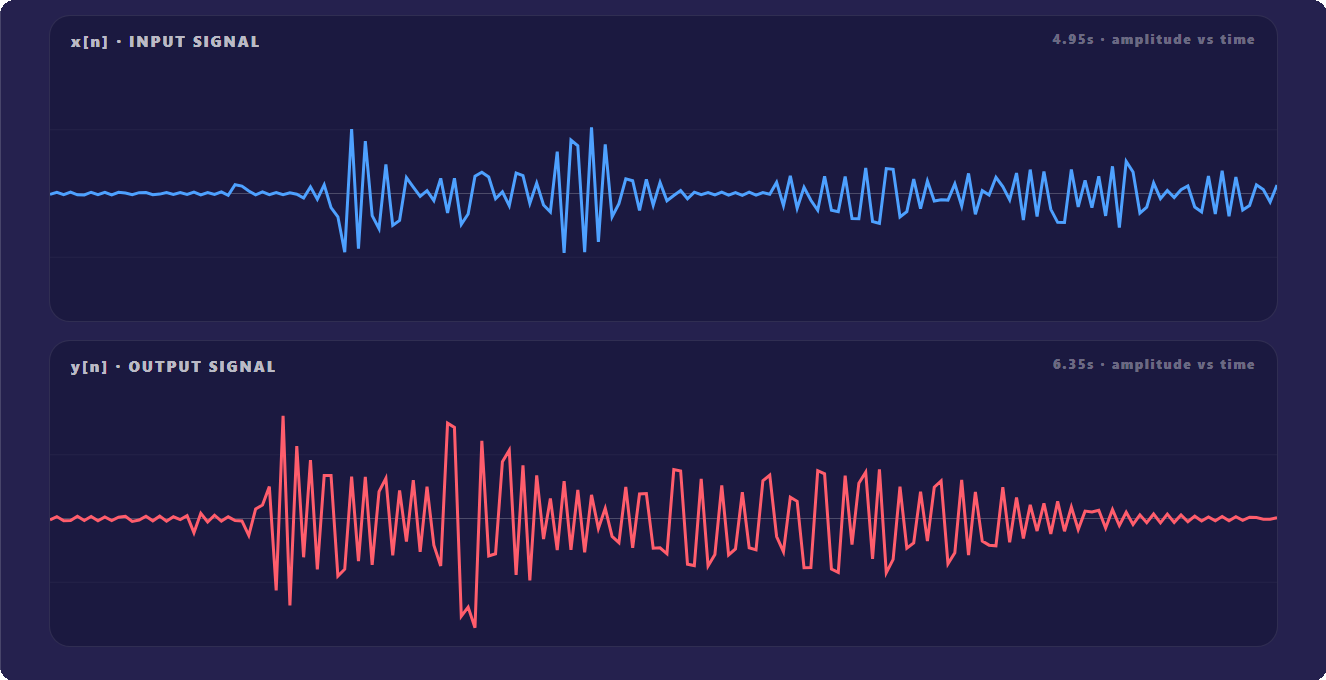
\includegraphics[width=\linewidth]{amp_io.png}\\[0.3em]
      \CaptionLine{Input $x[n]$ vs.\ output $y[n]$, $A=2$}
    \end{column}
  \end{columns}
\end{frame}

% ============================================================ 2. CONVOLUTION
\begin{frame}
  \ModuleTitle{MODULE 02 \,\textbullet\, TIME-DOMAIN}{Convolution}
  \begin{columns}[T]
    \begin{column}{0.42\linewidth}
      \begin{block}{Algorithm}
        \footnotesize
        \begin{enumerate}
          \item Take the input $x[n]$ and an impulse response $h[n]$ (e.g.\ a room's echo signature).
          \item \textbf{Reverse} $h$ in time.
          \item \textbf{Slide} the reversed $h$ across $x$, one sample shift at a time.
          \item At each shift, \textbf{multiply} the overlapping samples and \textbf{sum} them --- that sum is one output sample.
          \item Repeat until the reversed $h$ has slid completely past $x$.
        \end{enumerate}
      \end{block}
      \vspace{0.3em}
      \FormulaCard{\footnotesize$\displaystyle y[n] = \sum_{k} x[k]\,h[n-k]$}
      \vspace{0.2em}
      \CaptionLine{Computed via FFT convolution --- same sum, just fast.}
    \end{column}
    \begin{column}{0.56\linewidth}
      \centering
      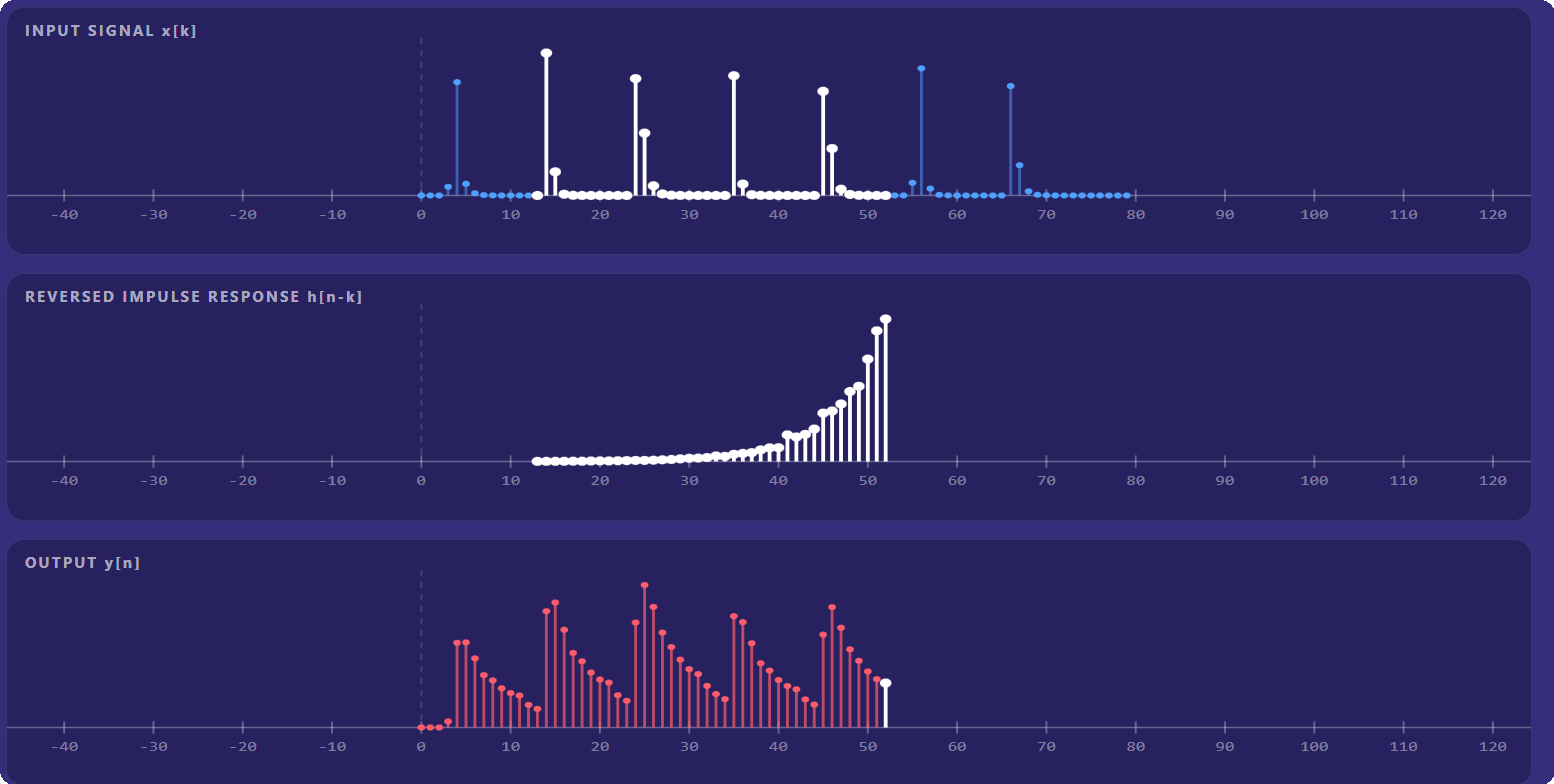
\includegraphics[width=\linewidth]{conv_viz.png}\\[0.3em]
      \CaptionLine{$x[k]$, reversed $h[n-k]$ sliding, and the accumulating output $y[n]$}
    \end{column}
  \end{columns}
\end{frame}

% ============================================================ 3. ECHO
\begin{frame}
  \ModuleTitle{MODULE 02 \,\textbullet\, TIME-DOMAIN}{Echo}
  \begin{columns}[T]
    \begin{column}{0.42\linewidth}
      \begin{block}{Algorithm --- feedback delay line}
        \footnotesize
        \begin{enumerate}
          \item Keep the original (dry) signal.
          \item Make a copy shifted later in time by $D$ samples, and shrink its volume by a decay factor $\alpha<1$.
          \item Add that quieter, delayed copy back into the output.
          \item \textbf{Repeat} steps 2--3 $R$ times: each new repeat is delayed further and decays more than the last (feedback).
          \item Sum every repeat with the original --- several decaying, evenly-spaced echoes.
        \end{enumerate}
      \end{block}
      \vspace{0.1em}
      \FormulaCard{\footnotesize$y[n]=x[n]+\sum_{r=1}^{R}\alpha^{r}x[n-rD]$}
    \end{column}
    \begin{column}{0.53\linewidth}
      \centering
      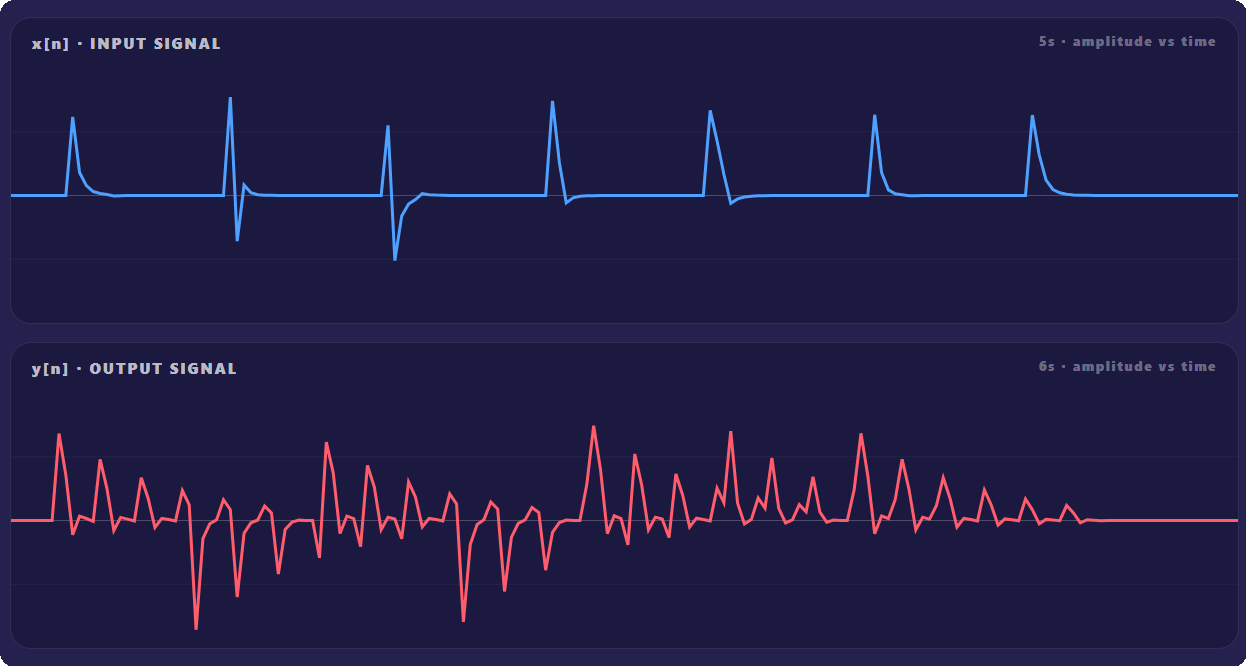
\includegraphics[width=\linewidth]{echo_io.png}\\[0.3em]
      \CaptionLine{Input $x[n]$ vs.\ output $y[n]$ --- repeated, decaying reflections}
    \end{column}
  \end{columns}
\end{frame}

% ============================================================ 4. DELAY
\begin{frame}
  \ModuleTitle{MODULE 02 \,\textbullet\, TIME-DOMAIN}{Delay}
  \begin{columns}[T]
    \begin{column}{0.42\linewidth}
      \begin{block}{Algorithm --- single repeat}
        \footnotesize
        \begin{enumerate}
          \item Keep the original (dry) signal.
          \item Make \textbf{one} copy shifted later in time by $D$ samples --- no feedback, it is not fed back into itself.
          \item Scale that single copy by a wet-mix factor $\alpha$.
          \item Add it to the original --- exactly one distinct, un-decayed repetition.
        \end{enumerate}
      \end{block}
      \vspace{0.4em}
      \FormulaCard{$y[n]=x[n]+\alpha\cdot x[n-D]$}
      \vspace{0.3em}
      \footnotesize Compare to Echo: same building block ($x[n-D]$), used once instead of looped.
    \end{column}
    \begin{column}{0.53\linewidth}
      \centering
      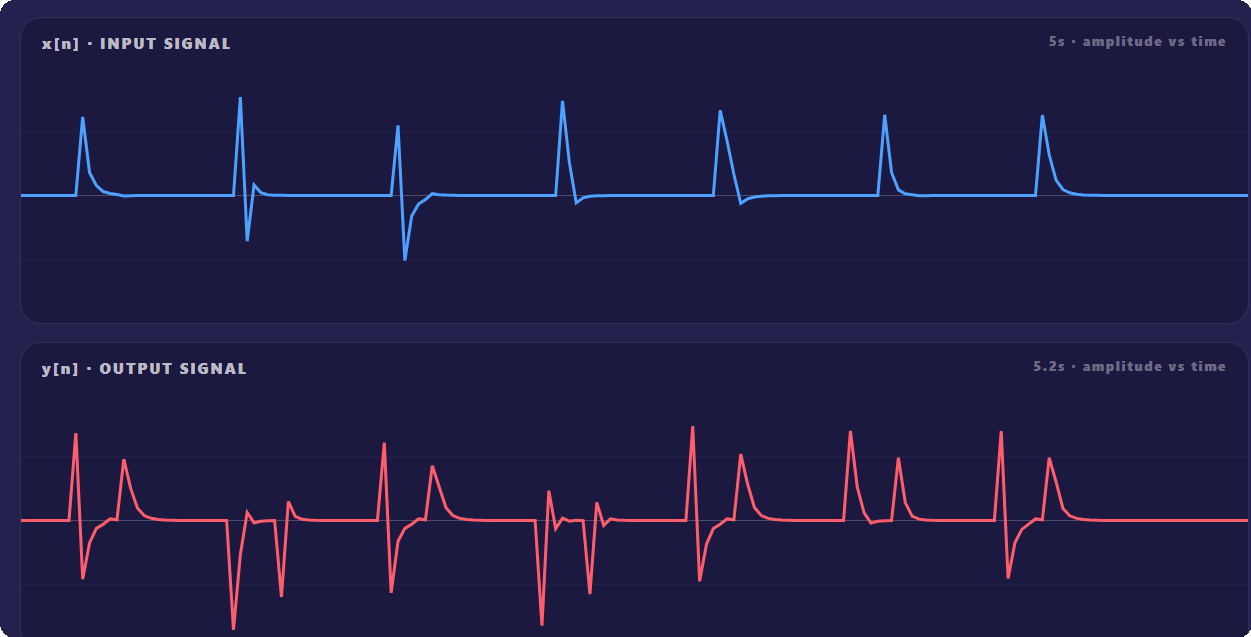
\includegraphics[width=\linewidth]{delay_io.png}\\[0.3em]
      \CaptionLine{Input $x[n]$ vs.\ output $y[n]$ --- one clean, delayed repeat}
    \end{column}
  \end{columns}
\end{frame}

% ============================================================ 5. SPECTRAL DETECTION
\begin{frame}
  \ModuleTitle{MODULE 03}{Spectral Detection --- Pitch}
  \begin{columns}[T]
    \begin{column}{0.44\linewidth}
      \begin{block}{Algorithm}
        \footnotesize
        \begin{enumerate}
          \item Apply a window (Hann) to the signal, then take its \textbf{FFT} to get the spectrum $|X(f)|$.
          \item Restrict the search to a chosen range $[f_{\min},f_{\max}]$ --- ignoring DC/rumble and inaudible highs.
          \item Find the frequency bin with the \textbf{largest magnitude} in that range --- the dominant frequency $f_0$.
          \item Map $f_0$ to the nearest musical note.
          \item \textbf{Synthesize} a pure sine wave at $f_0$ so the detection can be checked by ear.
        \end{enumerate}
      \end{block}
    \end{column}
    \begin{column}{0.53\linewidth}
      \centering
      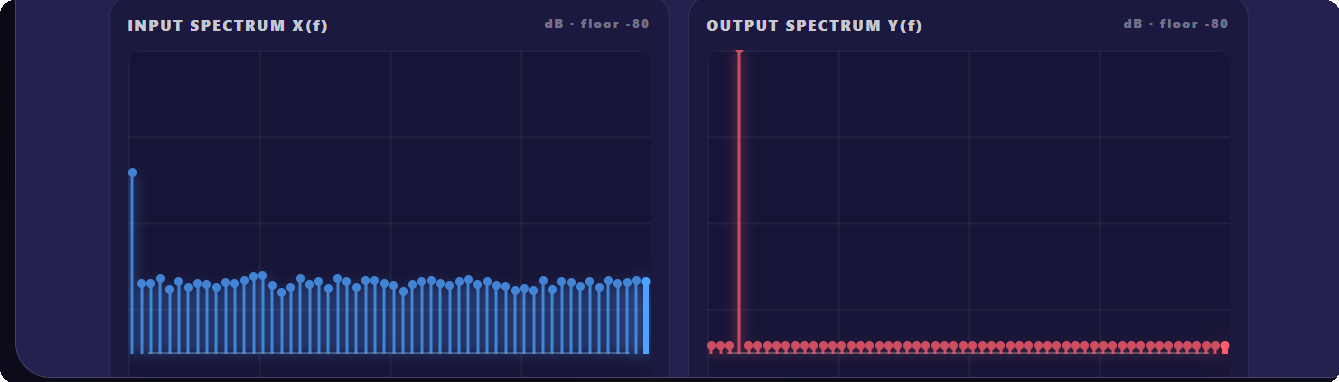
\includegraphics[width=\linewidth]{pitch_spectra.png}\\[0.3em]
      \FormulaCard{\footnotesize $f_0=\displaystyle\operatorname*{arg\,max}_{f\in[f_{\min},f_{\max}]}|X(f)|\quad$ $y[n]=A\sin(2\pi f_0 n/f_s)$}
      \CaptionLine{A real signal spreads energy across a fundamental \& overtones (left); the synthesized tone is one sharp spike at $f_0$ (right)}
    \end{column}
  \end{columns}
\end{frame}

% ============================================================ 6. SAMPLING & QUANTIZATION
\begin{frame}
  \ModuleTitle{MODULE 04}{Sampling \& Quantization}
  \begin{columns}[T]
    \begin{column}{0.5\linewidth}
      \centering
      \textbf{\small\color{blueAccent}Quantization}\\[0.2em]
      {\scriptsize
      \begin{enumerate}
        \item Pick how many bits $b$ to keep (e.g.\ 4-bit $=16$ levels).
        \item Compute the step size $\Delta$ spanning $[-1,1]$.
        \item \textbf{Round} each sample to the nearest allowed level, then clip.
      \end{enumerate}}
      \FormulaCard{\scriptsize $y[n]=\Delta\!\cdot\!\mathrm{round}(x[n]/\Delta),\;\Delta=\dfrac{2}{2^{b}-1}$}
      \vspace{0.15em}
      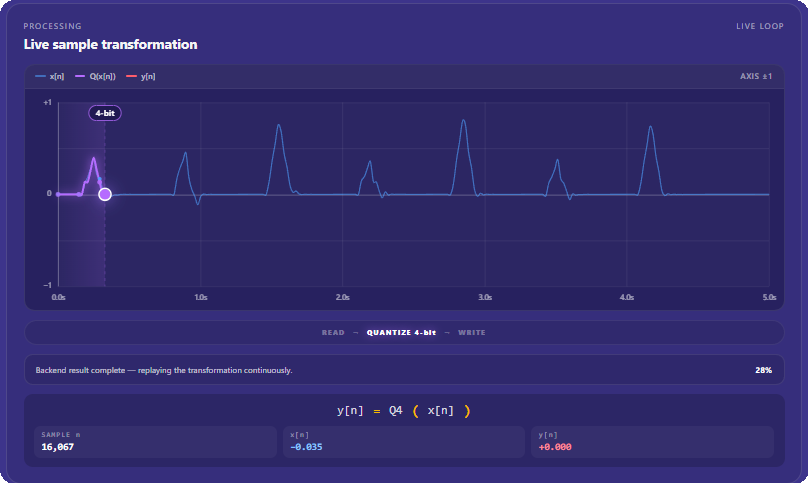
\includegraphics[width=0.72\linewidth]{quant_mid.png}
    \end{column}
    \begin{column}{0.5\linewidth}
      \centering
      \textbf{\small\color{redAccent}Sample-and-Hold}\\[0.2em]
      {\scriptsize
      \begin{enumerate}
        \item Pick a hold factor $N$ (simulates a lower sample rate).
        \item Walk the signal in blocks of $N$ samples.
        \item \textbf{Hold} the block's first sample for the whole block (zero-order hold), instead of reading a fresh one.
      \end{enumerate}}
      \FormulaCard{\scriptsize $y[n]=x\!\left(N\left\lfloor n/N\right\rfloor\right)$}
      \vspace{0.15em}
      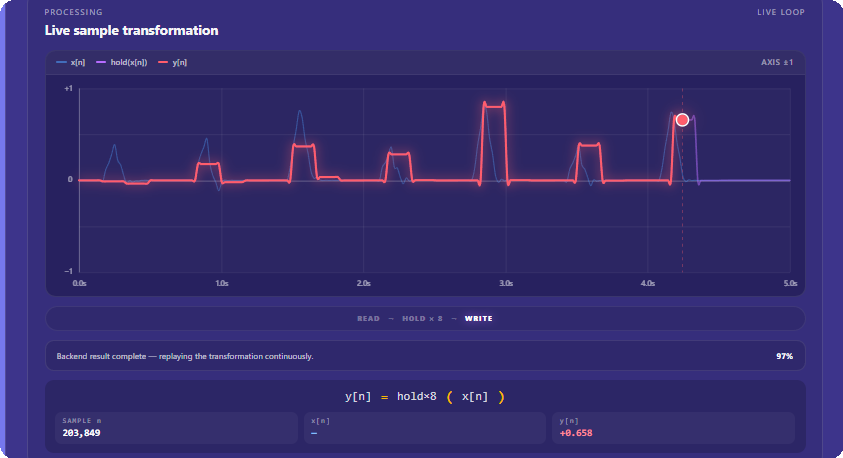
\includegraphics[width=0.72\linewidth]{sample_mid.png}
    \end{column}
  \end{columns}
\end{frame}

% ============================================================ 7. FILTERING
\begin{frame}
  \ModuleTitle{MODULE 05}{Frequency \& Filtering}
  \begin{columns}[T]
    \begin{column}{0.46\linewidth}
      \begin{block}{Algorithm}
        \scriptsize
        \begin{enumerate}
          \item Choose a filter family, band type, cutoff(s) and order $N$.
          \item \textbf{Design} the filter as \emph{SOS} (second-order sections): a chain of small 2-pole/2-zero stages multiplied together, instead of one giant high-order formula --- a high-order filter's raw coefficients can span a huge numeric range and go unstable; small cascaded stages stay well-behaved.
          \item \textbf{Apply it twice} with \texttt{sosfiltfilt}: once forwards, once backwards. The two passes cancel each other's phase delay, so output stays time-aligned with input.
        \end{enumerate}
      \end{block}
      \vspace{0.2em}
      \FormulaCard{\footnotesize $Y(f) = X(f)\cdot H(f)$}
    \end{column}
    \begin{column}{0.5\linewidth}
      \centering
      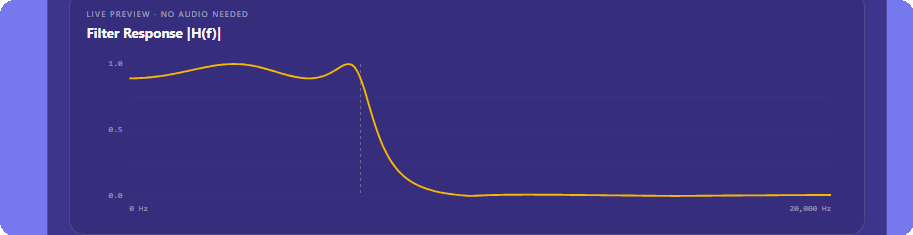
\includegraphics[width=\linewidth]{filter_response.png}\\[0.25em]
      \CaptionLine{The filter's own magnitude response $|H(f)|$ --- this lowpass example passes $f\le f_c$}
      \vspace{0.35em}
      \begin{block}{Families \& Bands}
        \scriptsize Butterworth \textbullet\; Chebyshev~I/II \textbullet\; Elliptic \textbullet\; Bessel \textbullet\; Ideal\\
        Lowpass \textbullet\; Highpass \textbullet\; Bandpass \textbullet\; Bandstop
      \end{block}
    \end{column}
  \end{columns}
\end{frame}

% ============================================================ 8. VOICE MORPHING
\begin{frame}
  \ModuleTitle{MODULE 06}{Voice Morphing --- Phase Vocoder}
  \begin{columns}[T]
    \begin{column}{0.48\linewidth}
      \begin{block}{Algorithm (Pitch / Time-Stretch)}
        \scriptsize
        \begin{enumerate}
          \item \textbf{STFT}: split into overlapping frames; get magnitude \& phase of each, independently.
          \item \textbf{Time-map}: to stretch by rate $r$, read analysis frames at $r\times$ the normal spacing (often between two real frames).
          \item \textbf{Magnitude interpolation}: blend the two nearest frames to estimate that in-between spectrum.
          \item \textbf{Phase updating}: estimate each bin's true frequency from the phase advance, then accumulate phase at the new spacing --- keeps frames coherent (the actual ``vocoder'' trick).
          \item Inverse-FFT \& overlap-add back to audio. \textbf{Pitch shift} then \textbf{resamples} to the original duration --- pitch moves, length returns to normal.
        \end{enumerate}
      \end{block}
    \end{column}
    \begin{column}{0.48\linewidth}
      \centering
      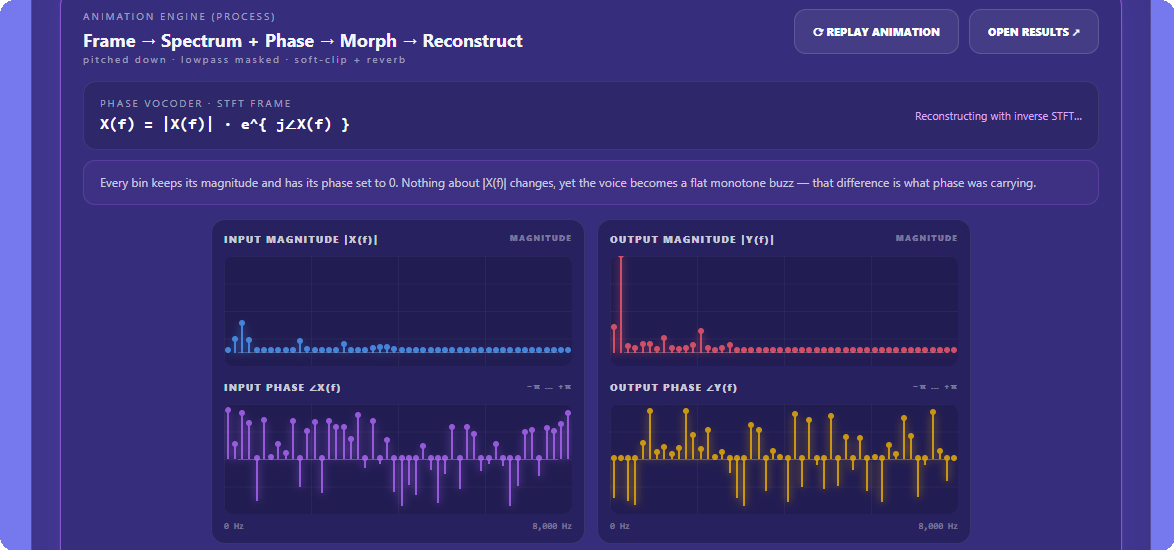
\includegraphics[width=\linewidth]{morph_panels.png}\\[0.3em]
      \FormulaCard{\scriptsize $X(f)=|X(f)|e^{j\angle X(f)}\;\;$\textbf{Robot}: $Y(f)=|X(f)|e^{j0}$}
      \scriptsize \textbf{Robot} skips all that: one STFT, phase forced to $0$, inverse-STFT --- magnitude survives, phase (voice's timing glue) does not. \textbf{Whisper} randomizes phase instead. Presets (Vader, Droid, Trooper, Cylon) layer pitch-shift/filter/ring-mod/reverb on top.
    \end{column}
  \end{columns}
\end{frame}

% ============================================================ 9. SPECTRAL PORTAL
\begin{frame}
  \ModuleTitle{MODULE 07}{Spectral Portal --- Spectrogram Masking}
  \begin{columns}[T]
    \begin{column}{0.44\linewidth}
      \begin{block}{Algorithm}
        \footnotesize
        \begin{enumerate}
          \item \textbf{Build the spectrogram}: windowed STFT frames give a time$\times$frequency grid; colour encodes $|X(k,m)|$ in dB (purple = quiet, gold = loud).
          \item \textbf{Paint KEEP/ERASE} rectangles $\to$ a binary mask $M(k,m)$, then Gaussian-blur it so edges are feathered, not a hard cut (avoids ringing).
          \item \textbf{Multiply} the mask into the complex spectrum, bin by bin.
          \item \textbf{Inverse STFT} (overlap--add) reconstructs the edited audio from what remains.
        \end{enumerate}
      \end{block}
      \vspace{0.25em}
      \FormulaCard{\footnotesize $X'(k,m)=M(k,m)\cdot X(k,m)$}
    \end{column}
    \begin{column}{0.53\linewidth}
      \centering
      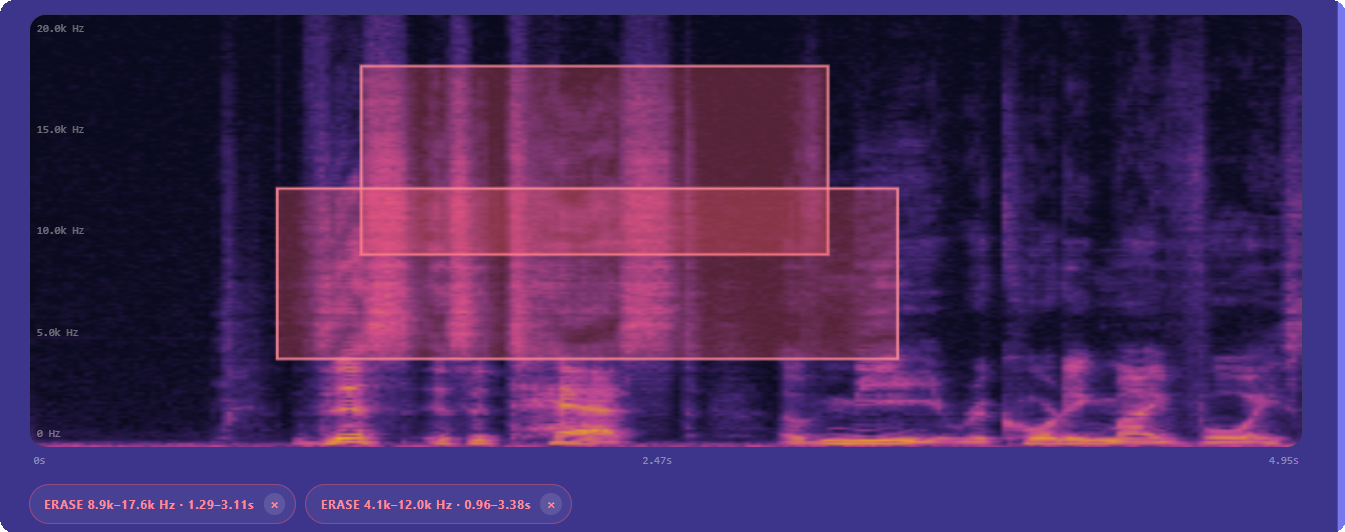
\includegraphics[width=\linewidth]{spectrogram_mask.png}\\[0.4em]
      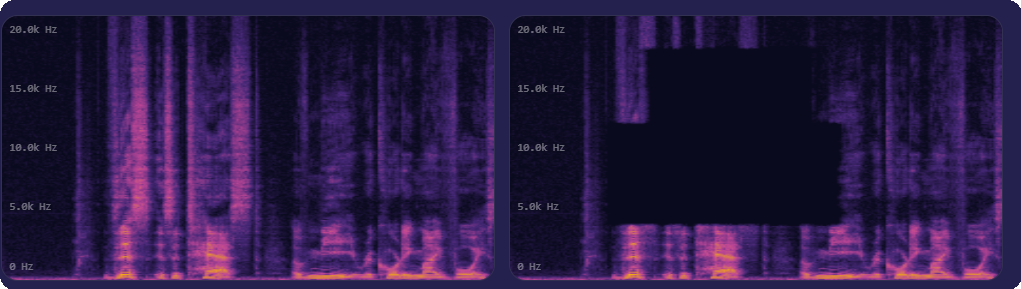
\includegraphics[width=\linewidth]{spectrogram_before_after.png}\\[0.2em]
      \CaptionLine{Drawn erase regions (top) $\rightarrow$ masked spectrogram, before/after (bottom)}
    \end{column}
  \end{columns}
\end{frame}

% ============================================================ 10. STUDIO
\begin{frame}
  \ModuleTitle{STUDIO}{Multi-Operation Signal Chain}
  \begin{columns}[T]
    \begin{column}{0.42\linewidth}
      \begin{block}{Algorithm}
        \footnotesize
        \begin{enumerate}
          \item Upload or record one input signal.
          \item Add effect steps to a chain, in any order (up to 25).
          \item Run the chain: each step's \textbf{output becomes the next step's input}.
          \item Inspect per-step timing/levels, and compare runs in history.
        \end{enumerate}
      \end{block}
      \vspace{0.3em}
      \FormulaCard{\footnotesize $y[n]=f_K\!\big(f_{K-1}(\cdots f_1(x[n])\cdots)\big)$}
    \end{column}
    \begin{column}{0.55\linewidth}
      \centering
      \resizebox{0.98\linewidth}{!}{%
      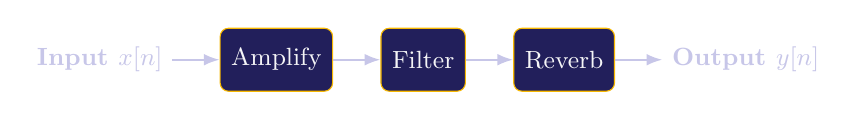
\begin{tikzpicture}[
          node distance=6mm,
          box/.style={draw=goldAccent, fill=cardBg, rounded corners=3pt, minimum height=8mm, text=textLight, font=\small, align=center, inner sep=4pt},
          io/.style={draw=none, fill=none, text=textMuted, font=\small\bfseries},
          arr/.style={-{Latex[length=2mm]}, draw=textMuted, thick}
        ]
        \node[io] (in) {Input $x[n]$};
        \node[box, right=of in] (a) {Amplify};
        \node[box, right=of a] (b) {Filter};
        \node[box, right=of b] (c) {Reverb};
        \node[io, right=of c] (out) {Output $y[n]$};
        \draw[arr] (in) -- (a);
        \draw[arr] (a) -- (b);
        \draw[arr] (b) -- (c);
        \draw[arr] (c) -- (out);
      \end{tikzpicture}}\\[1.2em]
      \small\color{textMuted} Any of the 7 modules' effects can be a step --- reorder, add, or remove freely.
    \end{column}
  \end{columns}
\end{frame}

% ============================================================ CONCLUSION
\begin{frame}
  \ModuleTitle{CONCLUSION}{Tech Stack \& Summary}
  \begin{columns}[T]
    \begin{column}{0.48\linewidth}
      \begin{block}{Backend Engine}
        \small Python \textbullet\; FastAPI \textbullet\; NumPy \textbullet\; SciPy \textbullet\; Librosa \textbullet\; soundfile
      \end{block}
      \vspace{0.4em}
      \begin{block}{Frontend Interaction}
        \small React \textbullet\; Vite \textbullet\; Modern CSS3 \textbullet\; Canvas-based live visualizations
      \end{block}
    \end{column}
    \begin{column}{0.48\linewidth}
      \begin{block}{DSP Methods Covered}
        \small FFT \& Spectrograms \textbullet\; Convolution \textbullet\; IIR/FIR Filtering \textbullet\; Quantization \& Aliasing \textbullet\; Phase Vocoder \textbullet\; Spectral Masking
      \end{block}
    \end{column}
  \end{columns}
  \vspace{1.2em}
  \centering
  {\large\color{goldAccent}\bfseries Thank You}\\[0.3em]
  {\small\color{textMuted} Md Mostakim (2305063) \quad\textbullet\quad Samiul Basir Adry (2305071)}
\end{frame}

\end{document}
